\section{Breadth-First Search (BFS) (Breitensuche)}
\begin{itemize}
    \item eine generelle Technik für die Traversierung eines Graphen
    \item besucht alle Vertizes und alle Kanten von G
    \item bestimmt, ob G verbunden ist
    \item berechnet / bestimmt die verbundene Komponenten von G
    \item berechnet einen aufspannenden Wald von G
    \item kann man auch erweitern, um andere Graphenprobleme zu lösen
    \begin{itemize}
        \item Finden und Ausgeben eines Pfades mit einer minimalen Anzahl Kanten zwischen zwei gegebenen Vertizes
        \item Finden von einfachen Zyklen
    \end{itemize}
\end{itemize}


\subsection{Laufzeit}
\begin{itemize}
    \item auf einem Graphen mit n Vertizes und m Kanten benötigt O(n + m) Zeit
    \item Setzen/Lesen eines Vertex-/Kanten-Labels benötigt O(1) Zeit
    \item Jeder Vertex wird zweifach markiert
    \begin{itemize}
        \item einmal als UNEXPLORED
        \item einmal als VISITED
    \end{itemize}
    \item Jede Kante wird zweifach markiert
    \begin{itemize}
        \item einmal als UNEXPLORED
        \item einmal als DISCOVERY oder CROSS
    \end{itemize}
    \item Die Methode incidentEdges() wird einmal pro Vertex aufgerufen
\end{itemize}


\subsection{Algorithmus}
\begin{center}
    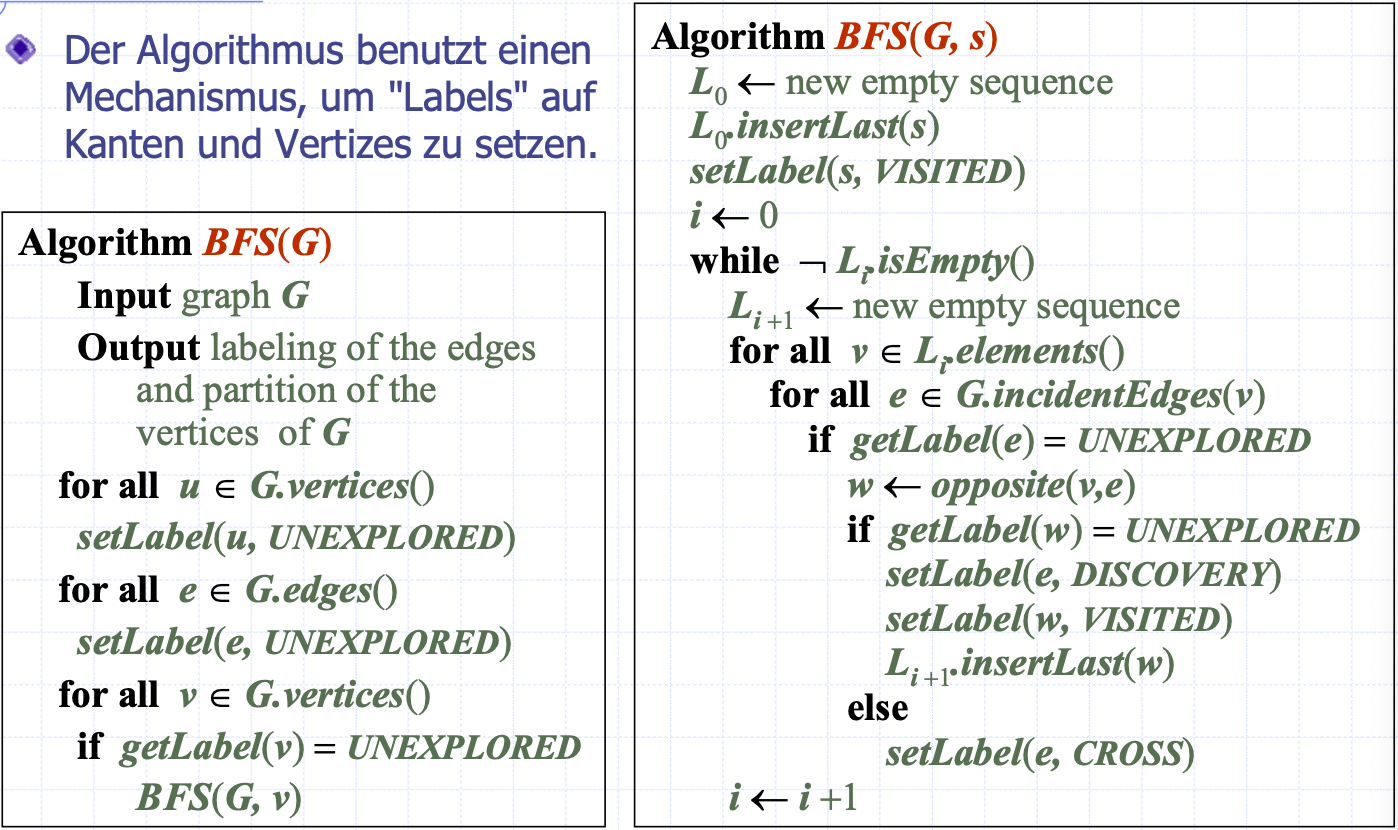
\includegraphics[scale=.25]{graphic/13 BFS/Algorithmus.png}
\end{center}
\vspace{-8pt}




\subsection{Beispiel}
\begin{center}
    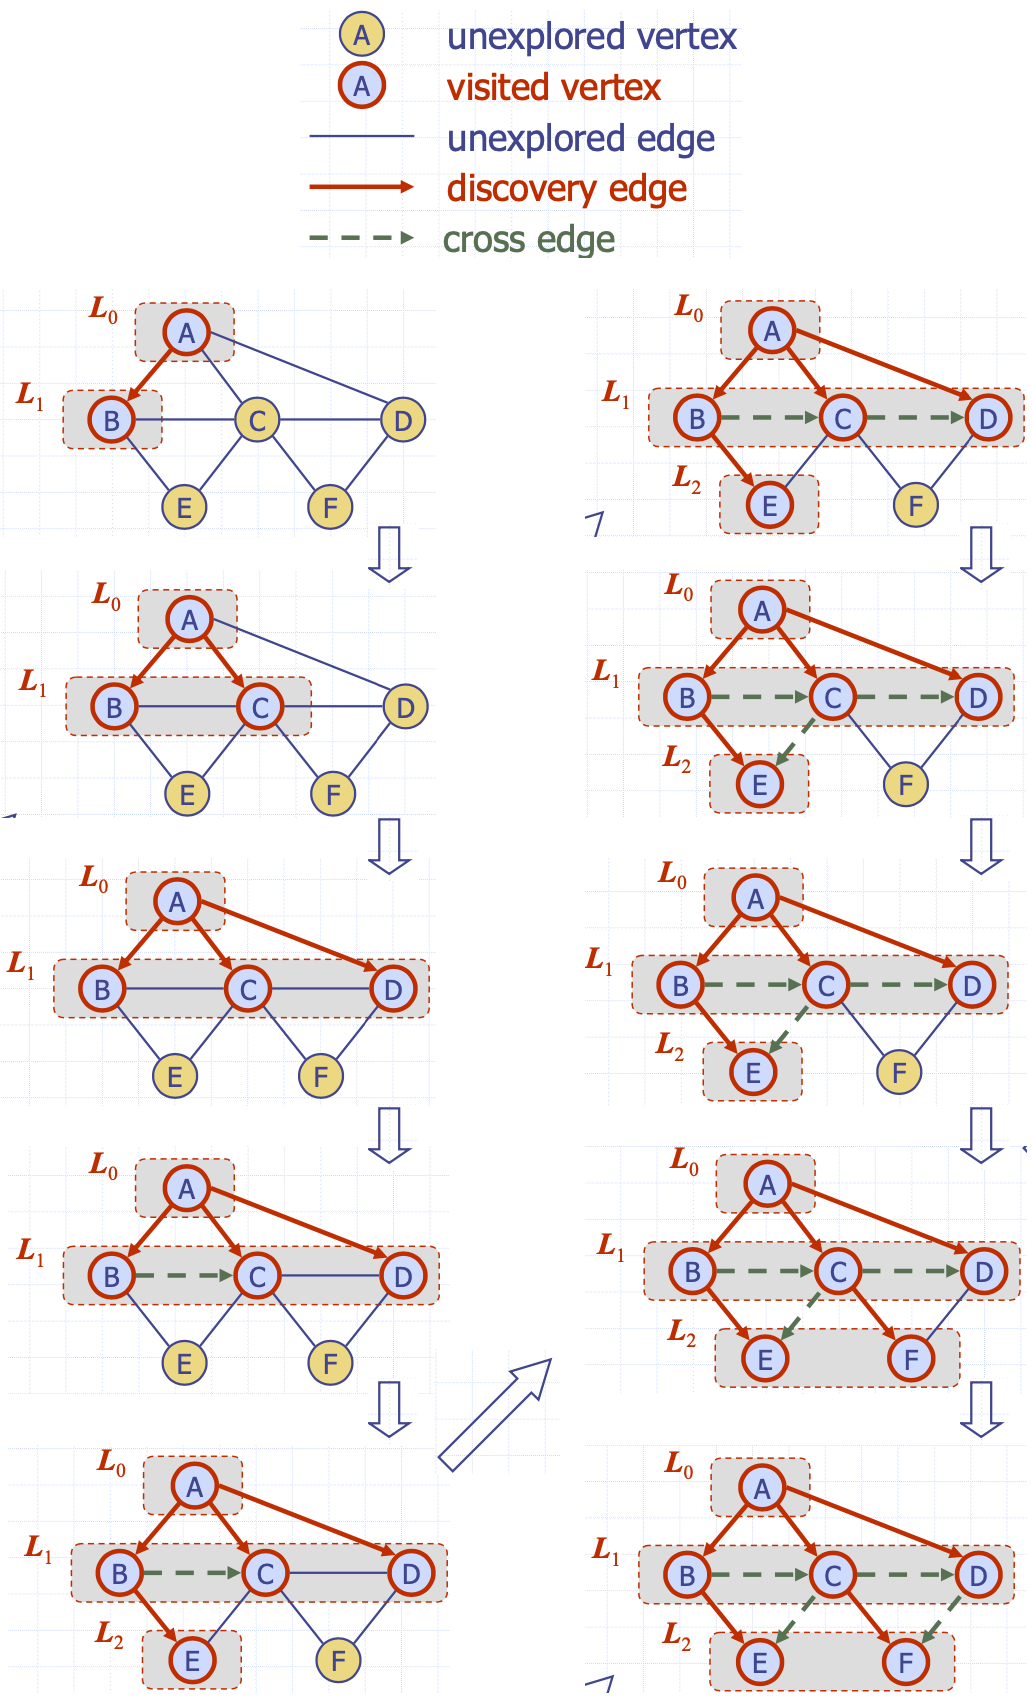
\includegraphics[scale=.3]{graphic/13 BFS/bsp.png}
\end{center}
\vspace{-8pt}

\subsection{Eigenschaften}
\begin{itemize}
    \item \textbf{Notation:}
    \begin{itemize}
        \item s = Start-Vertex
        \item $G_s$: verbundene Komponente von s
    \end{itemize}
    \item \textbf{Eigenschaft 1:}
    \begin{itemize}
        \item BFS(G, s) besucht alle Vertizes und Kanten in $G_s$
    \end{itemize}
    \item \textbf{Eigenschaft 2:}
    \begin{itemize}
        \item Die Discovery-Kanten von BFS(G, s) bilden einen aufspannenden Baum $T_s$ von $G_s$
    \end{itemize}
    \item \textbf{Eigenschaft 2:}\\
    für jeden Vertex v in Li gilt:
    \begin{itemize}
        \item der Pfad in $T_s$ von s nach v besitzt i Kanten
        \item Jeder Pfad von s nach v in $G_s$ besitzt mindestens i Kanten
    \end{itemize}
\end{itemize}

\subsection{Anwendungen}
\begin{itemize}
    \item bestimmen der verbundenen Komponenten von G
    \item bestimmen eines aufspannenden Waldes von G
    \item bestimmen eines einfachen Zyklus in G, oder bestimmen, ob G ein Wald ist
    \item bei zwei gegebenen Vertizes von G: finden eines Pfades in G zwischen den beiden Vertizes mit minimaler Anzahl Kanten oder bestimmen, ob ein solcher Pfad existiert
\end{itemize}
\subsection{DFS vs. BFS}
\begin{center}
    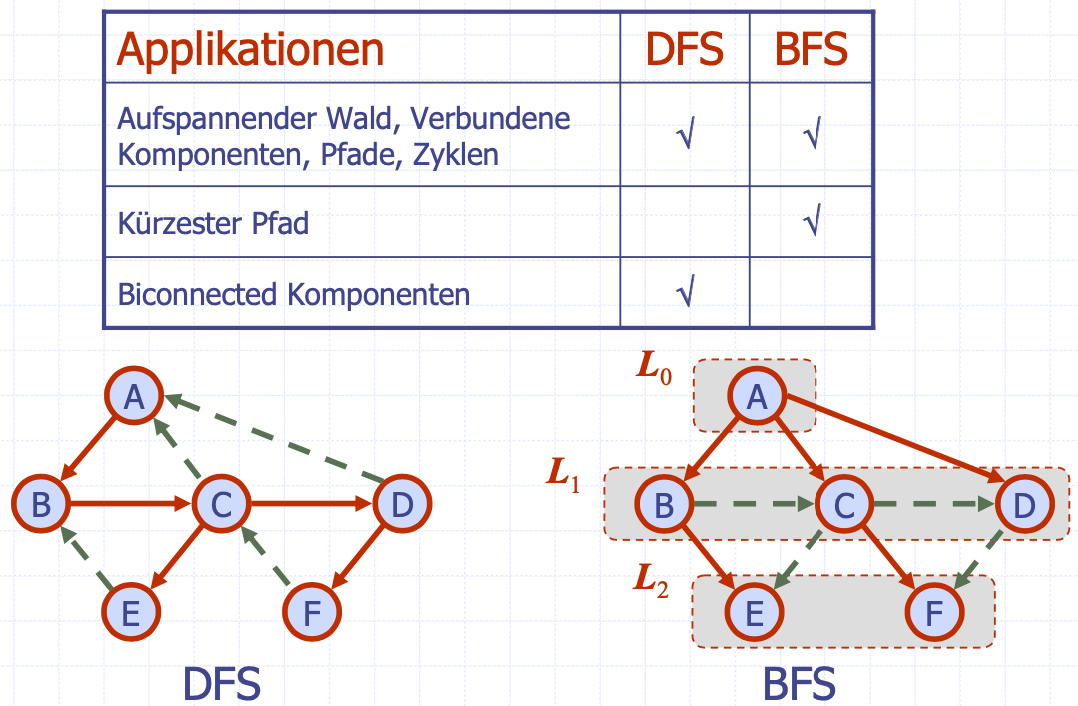
\includegraphics[scale=.25]{graphic/13 BFS/DFS vs. BFS1.png}
    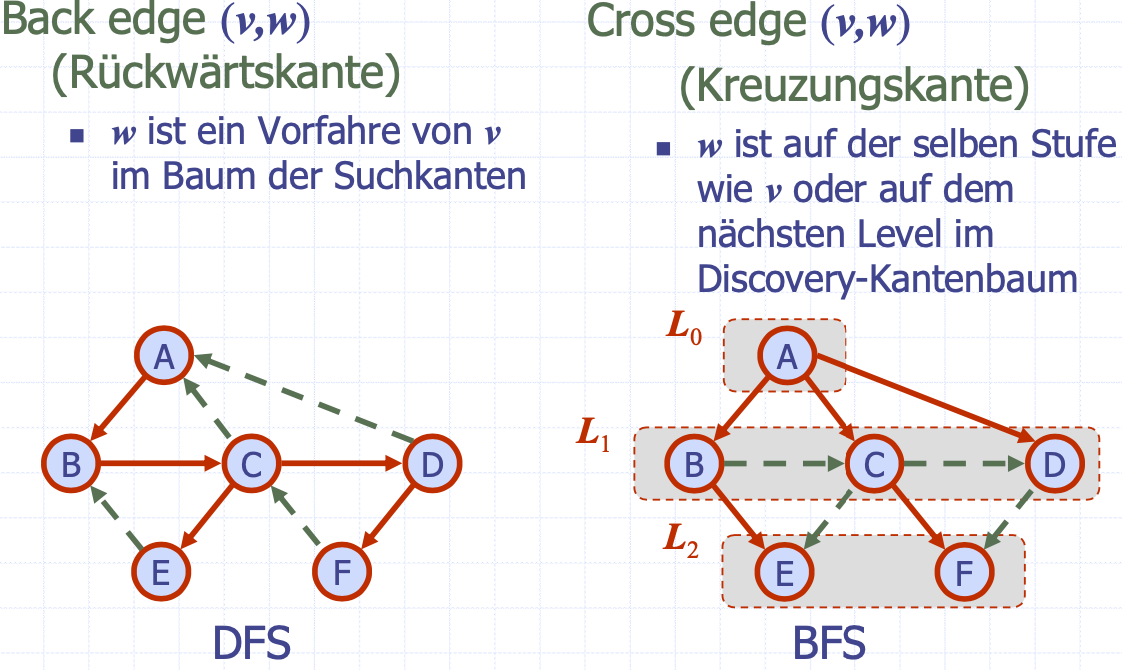
\includegraphics[scale=.25]{graphic/13 BFS/DFS vs. BFS2.png}
\end{center}
\vspace{-8pt}

\vfill
$ $
\columnbreak
\paragraph{Breitensuche}
\begin{center}
    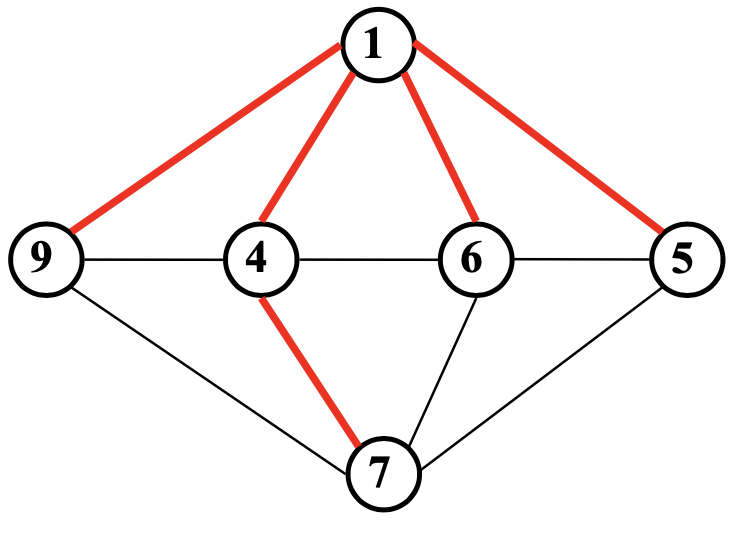
\includegraphics[scale=.25]{graphic/13 BFS/breitensuche.png}
\end{center}

\paragraph{Kürzester Pfad}
\begin{enumerate}
    \item Start Bei A
    \item Alle Distanzen = $\infty$, ausser direkt verbundene $\rightarrow$ Einzeichnen!
    \item Kürzeste Distanz verbinden (hier B)
    \item neue Distanzen einfügen
    \item Ab Schritt 3 wiederholen
\end{enumerate}
\begin{center}
    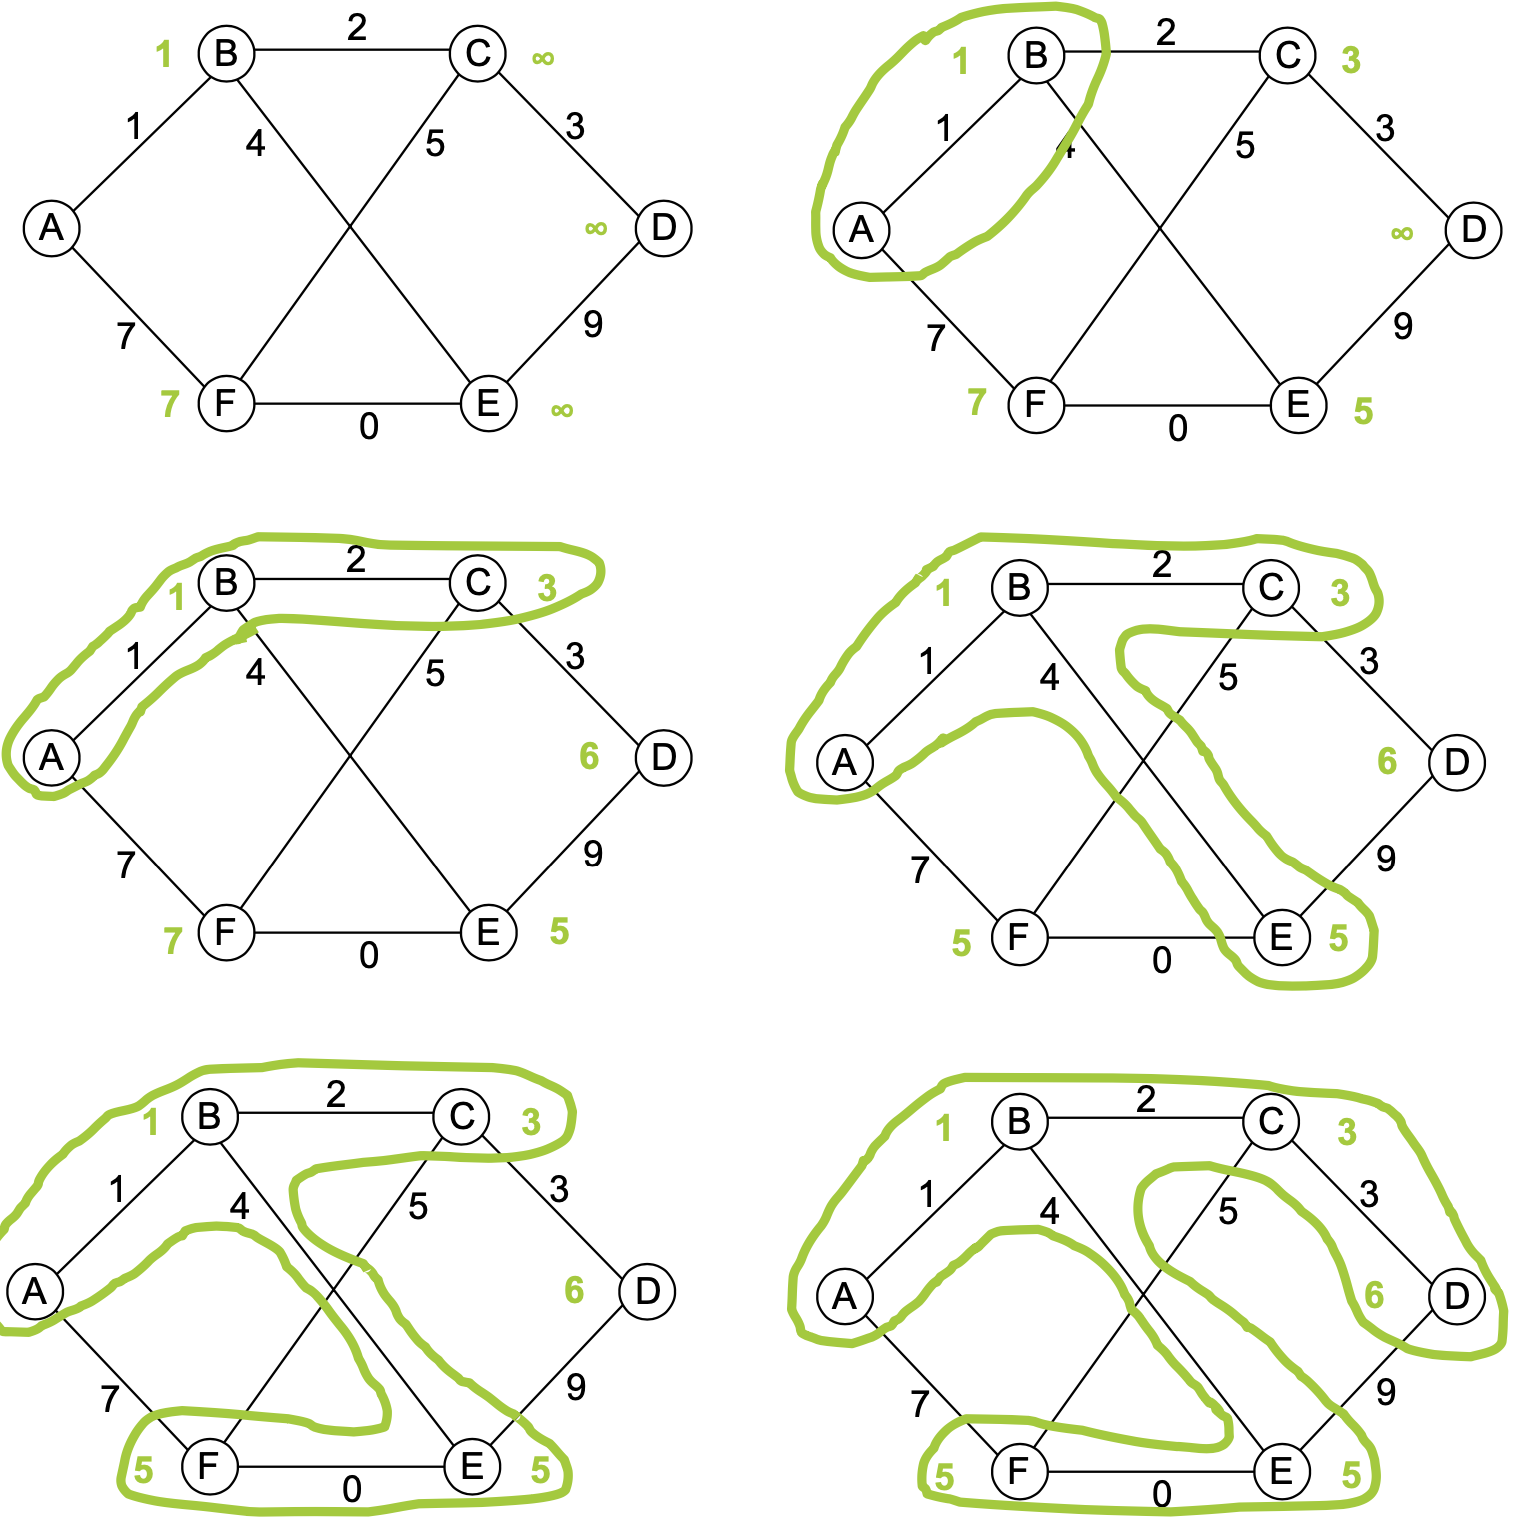
\includegraphics[scale=.25]{13 BFS/Kuerzester Pfad.png}
\end{center}
\newpage